\documentclass[12pt,a4paper]{article}
\usepackage[utf8]{inputenc}
\usepackage{amsmath}
\usepackage{amsfonts}
\usepackage{amssymb}
\usepackage{graphicx}
\author{José Antonio García Hernández}
\title{$d$-dimensional random walk}
\begin{document}
\maketitle

We present simulation results for the $d$-dimensional random walk. A random walker starts at the origin. The probability of moving in any direction in $d$ dimensions is $\frac{1}{2d}$. We let a random walker to take $N$ steps and finish the simulation if the walker ever reaches the origin again. We plotted the probability of a random walker to return to the origin in at least $N$ steps. We study the cases $d = 1,2,3,4,5$. 

\begin{center}
\begin{figure}
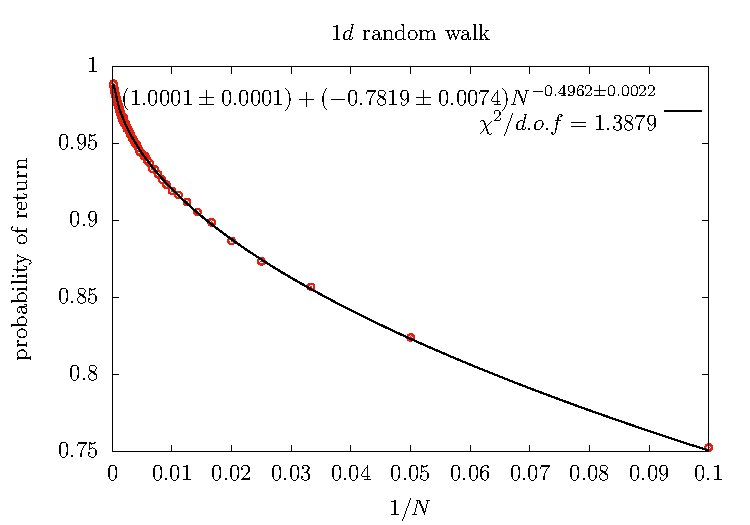
\includegraphics[scale=1]{1d_random_walk.pdf}
\caption{The probability at $N\to \infty$ is consistent with $1$ as the theroy predicts.}
\end{figure}
\end{center}


\begin{center}
\begin{figure}
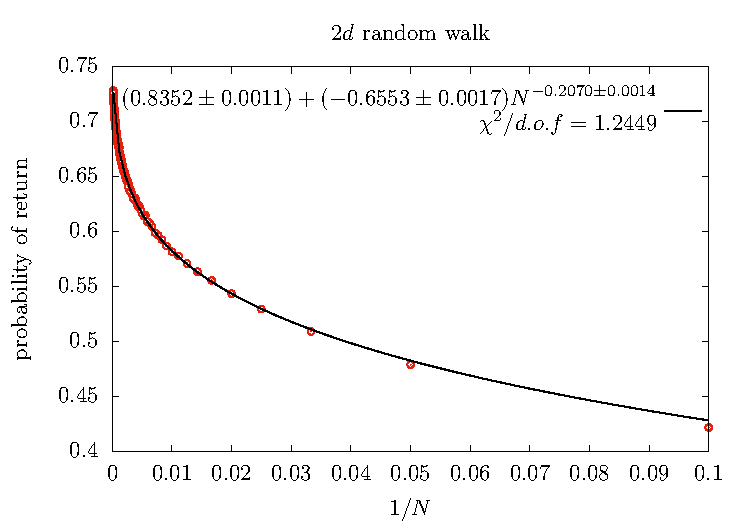
\includegraphics[scale=1]{2d_random_walk.pdf}
\end{figure}
\end{center}


\begin{center}
\begin{figure}
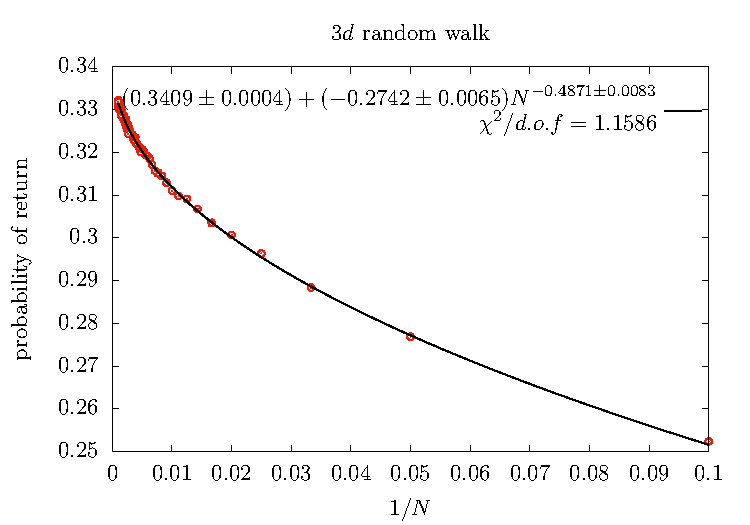
\includegraphics[scale=1]{3d_random_walk.pdf}
\end{figure}
\end{center}


\begin{center}
\begin{figure}
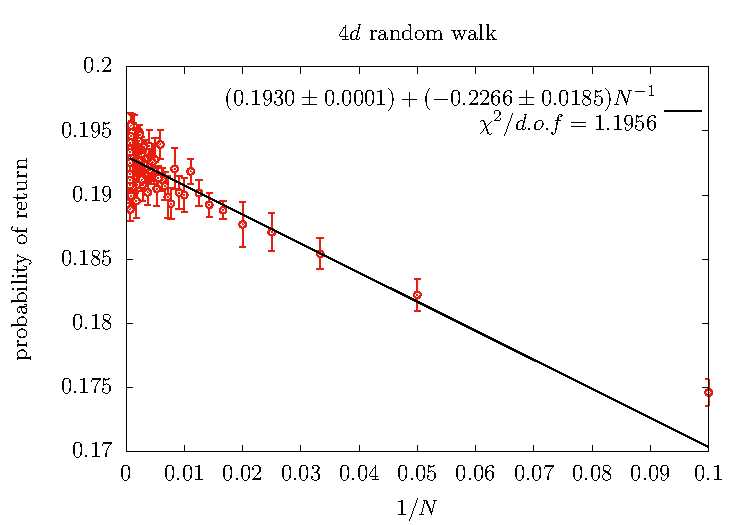
\includegraphics[scale=1]{4d_random_walk.pdf}
\end{figure}
\end{center}


\begin{center}
\begin{figure}
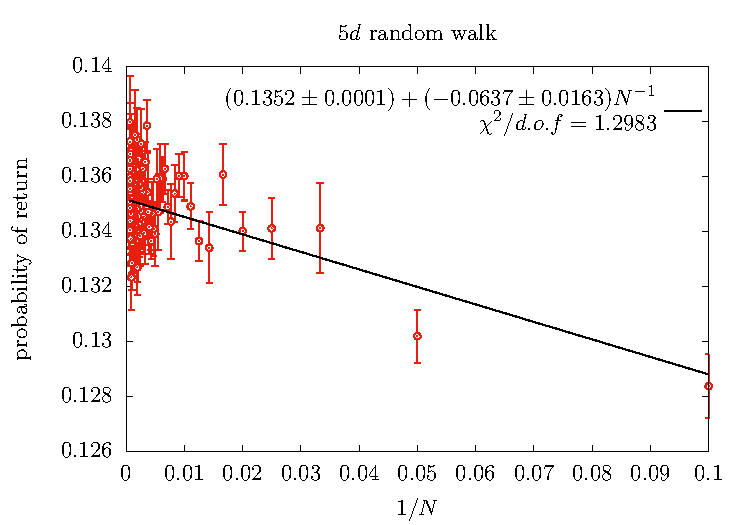
\includegraphics[scale=1]{5d_random_walk.pdf}
\end{figure}
\end{center}
\end{document}
